\documentclass[1p]{elsarticle_modified}
%\bibliographystyle{elsarticle-num}

%\usepackage[colorlinks]{hyperref}
%\usepackage{abbrmath_seonhwa} %\Abb, \Ascr, \Acal ,\Abf, \Afrak
\usepackage{amsfonts}
\usepackage{amssymb}
\usepackage{amsmath}
\usepackage{amsthm}
\usepackage{scalefnt}
\usepackage{amsbsy}
\usepackage{kotex}
\usepackage{caption}
\usepackage{subfig}
\usepackage{color}
\usepackage{graphicx}
\usepackage{xcolor} %% white, black, red, green, blue, cyan, magenta, yellow
\usepackage{float}
\usepackage{setspace}
\usepackage{hyperref}

\usepackage{tikz}
\usetikzlibrary{arrows}

\usepackage{multirow}
\usepackage{array} % fixed length table
\usepackage{hhline}

%%%%%%%%%%%%%%%%%%%%%
\makeatletter
\renewcommand*\env@matrix[1][\arraystretch]{%
	\edef\arraystretch{#1}%
	\hskip -\arraycolsep
	\let\@ifnextchar\new@ifnextchar
	\array{*\c@MaxMatrixCols c}}
\makeatother %https://tex.stackexchange.com/questions/14071/how-can-i-increase-the-line-spacing-in-a-matrix
%%%%%%%%%%%%%%%

\usepackage[normalem]{ulem}

\newcommand{\msout}[1]{\ifmmode\text{\sout{\ensuremath{#1}}}\else\sout{#1}\fi}
%SOURCE: \msout is \stkout macro in https://tex.stackexchange.com/questions/20609/strikeout-in-math-mode

\newcommand{\cancel}[1]{
	\ifmmode
	{\color{red}\msout{#1}}
	\else
	{\color{red}\sout{#1}}
	\fi
}

\newcommand{\add}[1]{
	{\color{blue}\uwave{#1}}
}

\newcommand{\replace}[2]{
	\ifmmode
	{\color{red}\msout{#1}}{\color{blue}\uwave{#2}}
	\else
	{\color{red}\sout{#1}}{\color{blue}\uwave{#2}}
	\fi
}

\newcommand{\Sol}{\mathcal{S}} %segment
\newcommand{\D}{D} %diagram
\newcommand{\A}{\mathcal{A}} %arc


%%%%%%%%%%%%%%%%%%%%%%%%%%%%%5 test

\def\sl{\operatorname{\textup{SL}}(2,\Cbb)}
\def\psl{\operatorname{\textup{PSL}}(2,\Cbb)}
\def\quan{\mkern 1mu \triangleright \mkern 1mu}

\theoremstyle{definition}
\newtheorem{thm}{Theorem}[section]
\newtheorem{prop}[thm]{Proposition}
\newtheorem{lem}[thm]{Lemma}
\newtheorem{ques}[thm]{Question}
\newtheorem{cor}[thm]{Corollary}
\newtheorem{defn}[thm]{Definition}
\newtheorem{exam}[thm]{Example}
\newtheorem{rmk}[thm]{Remark}
\newtheorem{alg}[thm]{Algorithm}

\newcommand{\I}{\sqrt{-1}}
\begin{document}

%\begin{frontmatter}
%
%\title{Boundary parabolic representations of knots up to 8 crossings}
%
%%% Group authors per affiliation:
%\author{Yunhi Cho} 
%\address{Department of Mathematics, University of Seoul, Seoul, Korea}
%\ead{yhcho@uos.ac.kr}
%
%
%\author{Seonhwa Kim} %\fnref{s_kim}}
%\address{Center for Geometry and Physics, Institute for Basic Science, Pohang, 37673, Korea}
%\ead{ryeona17@ibs.re.kr}
%
%\author{Hyuk Kim}
%\address{Department of Mathematical Sciences, Seoul National University, Seoul 08826, Korea}
%\ead{hyukkim@snu.ac.kr}
%
%\author{Seokbeom Yoon}
%\address{Department of Mathematical Sciences, Seoul National University, Seoul, 08826,  Korea}
%\ead{sbyoon15@snu.ac.kr}
%
%\begin{abstract}
%We find all boundary parabolic representation of knots up to 8 crossings.
%
%\end{abstract}
%\begin{keyword}
%    \MSC[2010] 57M25 
%\end{keyword}
%
%\end{frontmatter}

%\linenumbers
%\tableofcontents
%
\newcommand\colored[1]{\textcolor{white}{\rule[-0.35ex]{0.8em}{1.4ex}}\kern-0.8em\color{red} #1}%
%\newcommand\colored[1]{\textcolor{white}{ #1}\kern-2.17ex	\textcolor{white}{ #1}\kern-1.81ex	\textcolor{white}{ #1}\kern-2.15ex\color{red}#1	}

{\Large $\underline{11n_{181}~(K11n_{181})}$}

\setlength{\tabcolsep}{10pt}
\renewcommand{\arraystretch}{1.6}
\vspace{1cm}\begin{tabular}{m{100pt}>{\centering\arraybackslash}m{274pt}}
\multirow{5}{120pt}{
	\centering
	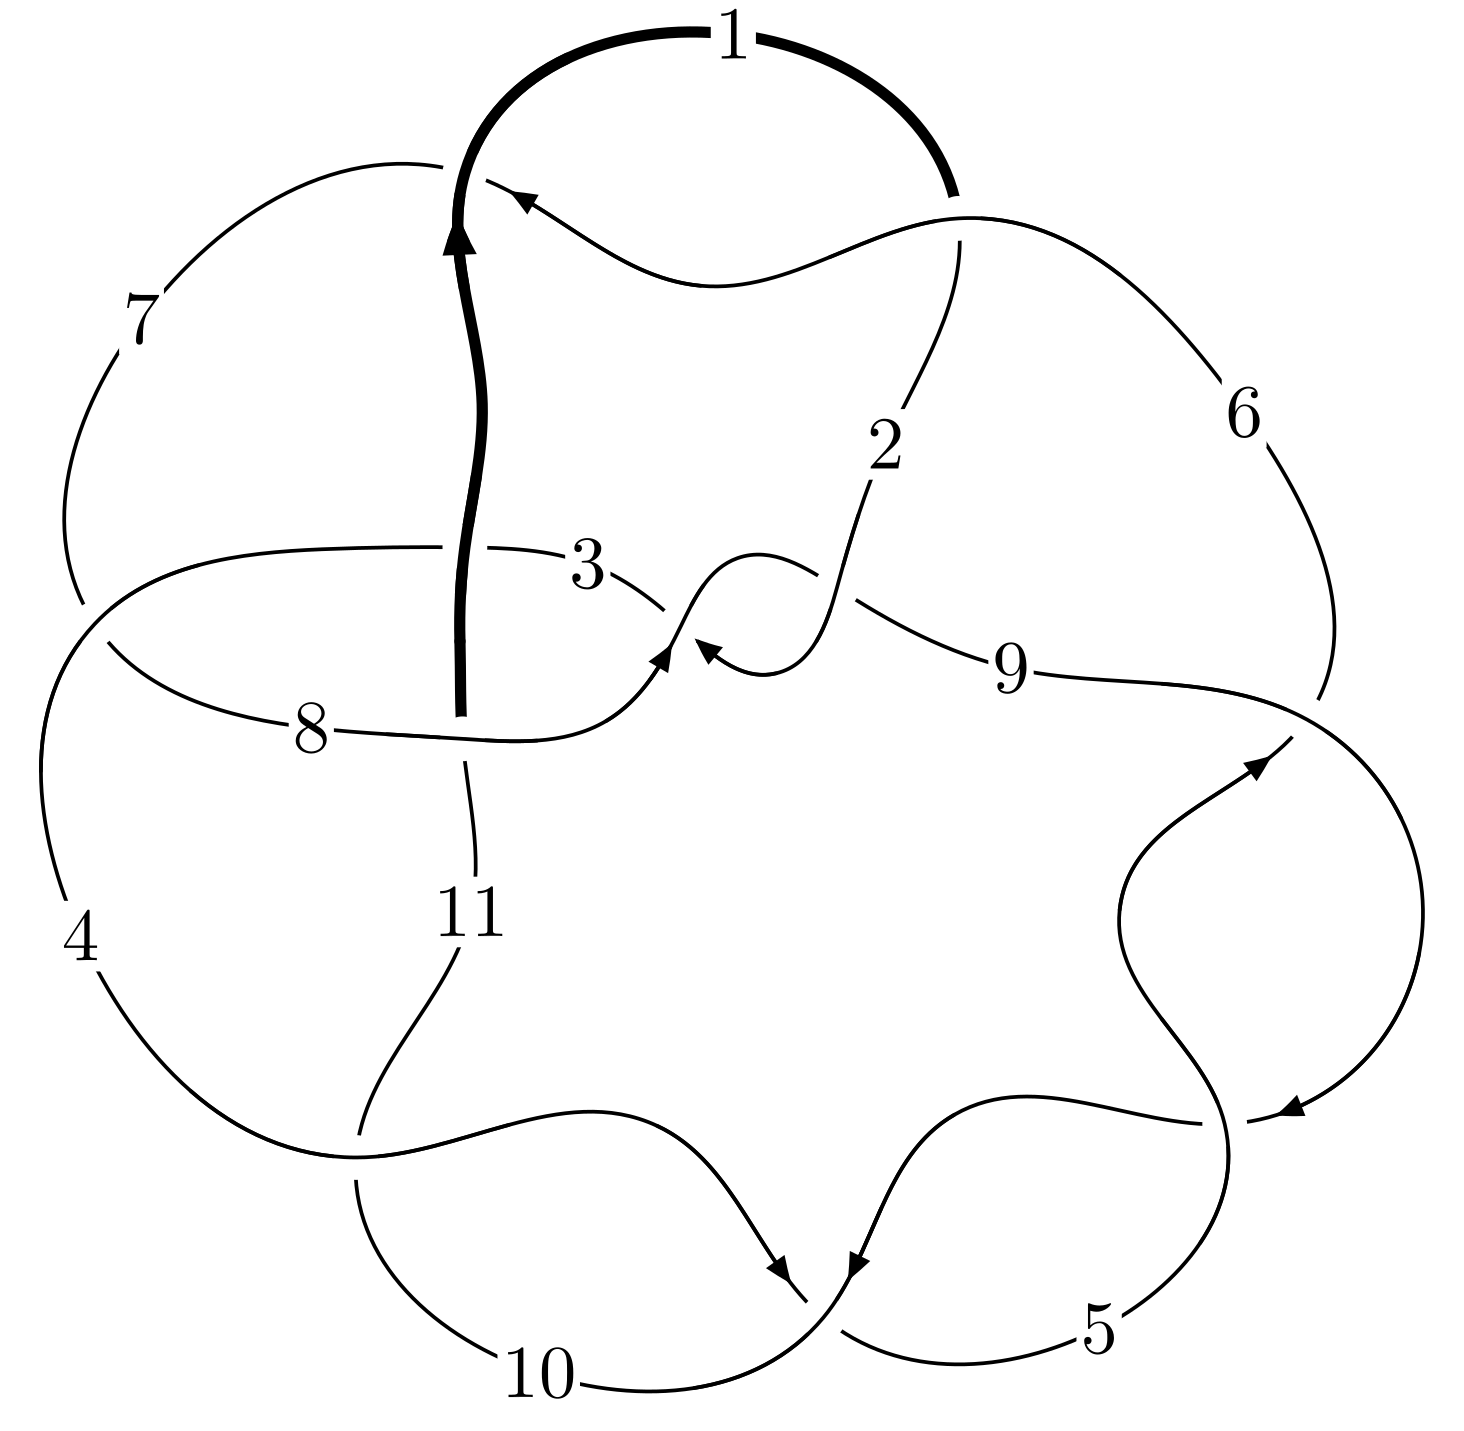
\includegraphics[width=112pt]{../../../GIT/diagram.site/Diagrams/png/797_11n_181.png}\\
\ \ \ A knot diagram\footnotemark}&
\allowdisplaybreaks
\textbf{Linearized knot diagam} \\
\cline{2-2}
 &
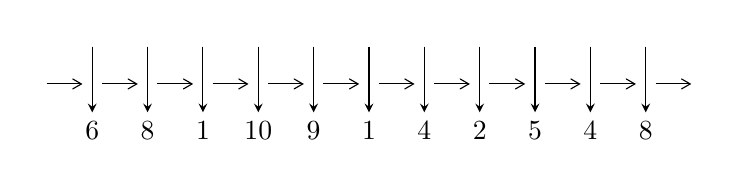
\begin{tikzpicture}[x=20pt, y=17pt]
	% nodes
	\node (C0) at (0, 0) {};
	\node (C1) at (1, 0) {};
	\node (C1U) at (1, +1) {};
	\node (C1D) at (1, -1) {6};

	\node (C2) at (2, 0) {};
	\node (C2U) at (2, +1) {};
	\node (C2D) at (2, -1) {8};

	\node (C3) at (3, 0) {};
	\node (C3U) at (3, +1) {};
	\node (C3D) at (3, -1) {1};

	\node (C4) at (4, 0) {};
	\node (C4U) at (4, +1) {};
	\node (C4D) at (4, -1) {10};

	\node (C5) at (5, 0) {};
	\node (C5U) at (5, +1) {};
	\node (C5D) at (5, -1) {9};

	\node (C6) at (6, 0) {};
	\node (C6U) at (6, +1) {};
	\node (C6D) at (6, -1) {1};

	\node (C7) at (7, 0) {};
	\node (C7U) at (7, +1) {};
	\node (C7D) at (7, -1) {4};

	\node (C8) at (8, 0) {};
	\node (C8U) at (8, +1) {};
	\node (C8D) at (8, -1) {2};

	\node (C9) at (9, 0) {};
	\node (C9U) at (9, +1) {};
	\node (C9D) at (9, -1) {5};

	\node (C10) at (10, 0) {};
	\node (C10U) at (10, +1) {};
	\node (C10D) at (10, -1) {4};

	\node (C11) at (11, 0) {};
	\node (C11U) at (11, +1) {};
	\node (C11D) at (11, -1) {8};
	\node (C12) at (12, 0) {};

	% arrows
	\draw[->,>={angle 60}]
	(C0) edge (C1) (C1) edge (C2) (C2) edge (C3) (C3) edge (C4) (C4) edge (C5) (C5) edge (C6) (C6) edge (C7) (C7) edge (C8) (C8) edge (C9) (C9) edge (C10) (C10) edge (C11) (C11) edge (C12) ;	\draw[->,>=stealth]
	(C1U) edge (C1D) (C2U) edge (C2D) (C3U) edge (C3D) (C4U) edge (C4D) (C5U) edge (C5D) (C6U) edge (C6D) (C7U) edge (C7D) (C8U) edge (C8D) (C9U) edge (C9D) (C10U) edge (C10D) (C11U) edge (C11D) ;
	\end{tikzpicture} \\
\hhline{~~} \\& 
\textbf{Solving Sequence} \\ \cline{2-2} 
 &
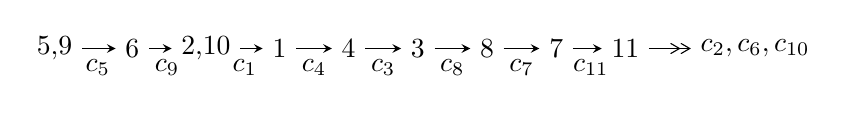
\begin{tikzpicture}[x=25pt, y=7pt]
	% node
	\node (A0) at (-1/8, 0) {5,9};
	\node (A1) at (1, 0) {6};
	\node (A2) at (33/16, 0) {2,10};
	\node (A3) at (25/8, 0) {1};
	\node (A4) at (33/8, 0) {4};
	\node (A5) at (41/8, 0) {3};
	\node (A6) at (49/8, 0) {8};
	\node (A7) at (57/8, 0) {7};
	\node (A8) at (65/8, 0) {11};
	\node (C1) at (1/2, -1) {$c_{5}$};
	\node (C2) at (3/2, -1) {$c_{9}$};
	\node (C3) at (21/8, -1) {$c_{1}$};
	\node (C4) at (29/8, -1) {$c_{4}$};
	\node (C5) at (37/8, -1) {$c_{3}$};
	\node (C6) at (45/8, -1) {$c_{8}$};
	\node (C7) at (53/8, -1) {$c_{7}$};
	\node (C8) at (61/8, -1) {$c_{11}$};
	\node (A9) at (10, 0) {$c_{2},c_{6},c_{10}$};

	% edge
	\draw[->,>=stealth]	
	(A0) edge (A1) (A1) edge (A2) (A2) edge (A3) (A3) edge (A4) (A4) edge (A5) (A5) edge (A6) (A6) edge (A7) (A7) edge (A8) ;
	\draw[->>,>={angle 60}]	
	(A8) edge (A9);
\end{tikzpicture} \\ 

\end{tabular} \\

\footnotetext{
The image of knot diagram is generated by the software ``\textbf{Draw programme}" developed by Andrew Bartholomew(\url{http://www.layer8.co.uk/maths/draw/index.htm\#Running-draw}), where we modified some parts for our purpose(\url{https://github.com/CATsTAILs/LinksPainter}).
}\phantom \\ \newline 
\centering \textbf{Ideals for irreducible components\footnotemark of $X_{\text{par}}$} 
 
\begin{align*}
I^u_{1}&=\langle 
u^{12}-5 u^{11}+18 u^{10}-47 u^9+95 u^8-157 u^7+208 u^6-225 u^5+194 u^4-129 u^3+62 u^2+2 b-19 u+2,\\
\phantom{I^u_{1}}&\phantom{= \langle  }u^{12}-3 u^{11}+14 u^{10}-31 u^9+73 u^8-119 u^7+178 u^6-209 u^5+208 u^4-165 u^3+104 u^2+4 a-45 u+12,\\
\phantom{I^u_{1}}&\phantom{= \langle  }u^{13}-5 u^{12}+\cdots+30 u-4\rangle \\
I^u_{2}&=\langle 
- a^3 u^3- a^3 u^2- a^3 u+a^2 u^2+u^3 a+a^2 u- u^3+a u- u^2+b+a-2 u+1,\\
\phantom{I^u_{2}}&\phantom{= \langle  }- a^3 u^3+u^3 a^2+a^4-2 a^3 u+6 u^3 a+2 a^2 u+5 u^2 a+4 u^3- a^2+15 a u+6 u^2+10 a+11 u+12,\\
\phantom{I^u_{2}}&\phantom{= \langle  }u^4+u^3+3 u^2+2 u+1\rangle \\
I^u_{3}&=\langle 
u^4+u^3+2 u^2+b+2 u,\;u^2+a+2,\;u^7+5 u^5+7 u^3+2 u-1\rangle \\
\\
\end{align*}
\raggedright * 3 irreducible components of $\dim_{\mathbb{C}}=0$, with total 36 representations.\\
\footnotetext{All coefficients of polynomials are rational numbers. But the coefficients are sometimes approximated in decimal forms when there is not enough margin.}
\newpage
\renewcommand{\arraystretch}{1}
\centering \section*{I. $I^u_{1}= \langle u^{12}-5 u^{11}+\cdots+2 b+2,\;u^{12}-3 u^{11}+\cdots+4 a+12,\;u^{13}-5 u^{12}+\cdots+30 u-4 \rangle$}
\flushleft \textbf{(i) Arc colorings}\\
\begin{tabular}{m{7pt} m{180pt} m{7pt} m{180pt} }
\flushright $a_{5}=$&$\begin{pmatrix}1\\0\end{pmatrix}$ \\
\flushright $a_{9}=$&$\begin{pmatrix}0\\u\end{pmatrix}$ \\
\flushright $a_{6}=$&$\begin{pmatrix}1\\u^2\end{pmatrix}$ \\
\flushright $a_{2}=$&$\begin{pmatrix}-\frac{1}{4} u^{12}+\frac{3}{4} u^{11}+\cdots+\frac{45}{4} u-3\\-\frac{1}{2} u^{12}+\frac{5}{2} u^{11}+\cdots+\frac{19}{2} u-1\end{pmatrix}$ \\
\flushright $a_{10}=$&$\begin{pmatrix}- u\\u\end{pmatrix}$ \\
\flushright $a_{1}=$&$\begin{pmatrix}\frac{1}{4} u^{12}-\frac{3}{4} u^{11}+\cdots+\frac{27}{4} u-2\\\frac{1}{2} u^{12}-\frac{5}{2} u^{11}+\cdots-\frac{37}{2} u+3\end{pmatrix}$ \\
\flushright $a_{4}=$&$\begin{pmatrix}u^2+1\\- u^2\end{pmatrix}$ \\
\flushright $a_{3}=$&$\begin{pmatrix}\frac{1}{2} u^{12}-2 u^{11}+\cdots-\frac{29}{2} u+\frac{7}{2}\\\frac{1}{2} u^{12}-\frac{5}{2} u^{11}+\cdots-\frac{31}{2} u+2\end{pmatrix}$ \\
\flushright $a_{8}=$&$\begin{pmatrix}u^{12}-\frac{9}{2} u^{11}+\cdots-28 u+\frac{9}{2}\\-\frac{1}{2} u^{12}+\frac{5}{2} u^{11}+\cdots+\frac{31}{2} u-2\end{pmatrix}$ \\
\flushright $a_{7}=$&$\begin{pmatrix}-\frac{1}{2} u^{12}+2 u^{11}+\cdots+\frac{5}{2} u+\frac{1}{2}\\\frac{1}{2} u^{12}-\frac{5}{2} u^{11}+\cdots-\frac{25}{2} u+2\end{pmatrix}$ \\
\flushright $a_{11}=$&$\begin{pmatrix}- u^3-2 u\\u^3+u\end{pmatrix}$\\ \flushright $a_{11}=$&$\begin{pmatrix}- u^3-2 u\\u^3+u\end{pmatrix}$\\&\end{tabular}
\flushleft \textbf{(ii) Obstruction class $= -1$}\\~\\
\flushleft \textbf{(iii) Cusp Shapes $= - u^{12}+5 u^{11}-20 u^{10}+54 u^9-121 u^8+212 u^7-314 u^6+374 u^5-372 u^4+295 u^3-186 u^2+88 u-34$}\\~\\
\newpage\renewcommand{\arraystretch}{1}
\flushleft \textbf{(iv) u-Polynomials at the component}\newline \\
\begin{tabular}{m{50pt}|m{274pt}}
Crossings & \hspace{64pt}u-Polynomials at each crossing \\
\hline $$\begin{aligned}c_{1},c_{2},c_{6}\\c_{8}\end{aligned}$$&$\begin{aligned}
&u^{13}+5 u^{11}+\cdots+2 u+1
\end{aligned}$\\
\hline $$\begin{aligned}c_{3}\end{aligned}$$&$\begin{aligned}
&u^{13}-12 u^{12}+\cdots-16 u+16
\end{aligned}$\\
\hline $$\begin{aligned}c_{4},c_{5},c_{9}\\c_{10}\end{aligned}$$&$\begin{aligned}
&u^{13}+5 u^{12}+\cdots+30 u+4
\end{aligned}$\\
\hline $$\begin{aligned}c_{7},c_{11}\end{aligned}$$&$\begin{aligned}
&u^{13}+u^{12}+\cdots+3 u+1
\end{aligned}$\\
\hline
\end{tabular}\\~\\
\newpage\renewcommand{\arraystretch}{1}
\flushleft \textbf{(v) Riley Polynomials at the component}\newline \\
\begin{tabular}{m{50pt}|m{274pt}}
Crossings & \hspace{64pt}Riley Polynomials at each crossing \\
\hline $$\begin{aligned}c_{1},c_{2},c_{6}\\c_{8}\end{aligned}$$&$\begin{aligned}
&y^{13}+10 y^{12}+\cdots+30 y^2-1
\end{aligned}$\\
\hline $$\begin{aligned}c_{3}\end{aligned}$$&$\begin{aligned}
&y^{13}-6 y^{12}+\cdots+4480 y-256
\end{aligned}$\\
\hline $$\begin{aligned}c_{4},c_{5},c_{9}\\c_{10}\end{aligned}$$&$\begin{aligned}
&y^{13}+15 y^{12}+\cdots+124 y-16
\end{aligned}$\\
\hline $$\begin{aligned}c_{7},c_{11}\end{aligned}$$&$\begin{aligned}
&y^{13}-17 y^{12}+\cdots+25 y-1
\end{aligned}$\\
\hline
\end{tabular}\\~\\
\newpage\flushleft \textbf{(vi) Complex Volumes and Cusp Shapes}
$$\begin{array}{c|c|c}  
\text{Solutions to }I^u_{1}& \I (\text{vol} + \sqrt{-1}CS) & \text{Cusp shape}\\
 \hline 
\begin{aligned}
u &= \phantom{-}0.144857 + 0.988588 I \\
a &= \phantom{-}0.636883 - 0.256528 I \\
b &= -0.881451 - 0.164723 I\end{aligned}
 & \phantom{-}2.39689 - 1.47210 I & -6.76905 + 4.68228 I \\ \hline\begin{aligned}
u &= \phantom{-}0.144857 - 0.988588 I \\
a &= \phantom{-}0.636883 + 0.256528 I \\
b &= -0.881451 + 0.164723 I\end{aligned}
 & \phantom{-}2.39689 + 1.47210 I & -6.76905 - 4.68228 I \\ \hline\begin{aligned}
u &= \phantom{-}0.698010 + 0.761843 I \\
a &= -1.308540 - 0.343629 I \\
b &= \phantom{-}1.138990 - 0.122915 I\end{aligned}
 & -1.53379 - 7.84030 I & -8.79484 + 6.42108 I \\ \hline\begin{aligned}
u &= \phantom{-}0.698010 - 0.761843 I \\
a &= -1.308540 + 0.343629 I \\
b &= \phantom{-}1.138990 + 0.122915 I\end{aligned}
 & -1.53379 + 7.84030 I & -8.79484 - 6.42108 I \\ \hline\begin{aligned}
u &= \phantom{-}0.853563 + 0.271566 I \\
a &= \phantom{-}0.142752 - 1.224120 I \\
b &= \phantom{-}0.206699 + 0.270697 I\end{aligned}
 & -3.02361 + 2.70878 I & -9.87229 - 2.50117 I \\ \hline\begin{aligned}
u &= \phantom{-}0.853563 - 0.271566 I \\
a &= \phantom{-}0.142752 + 1.224120 I \\
b &= \phantom{-}0.206699 - 0.270697 I\end{aligned}
 & -3.02361 - 2.70878 I & -9.87229 + 2.50117 I \\ \hline\begin{aligned}
u &= \phantom{-}0.360660 + 1.314350 I \\
a &= \phantom{-}0.518668 + 0.256927 I \\
b &= -0.921497 - 0.693070 I\end{aligned}
 & \phantom{-}1.92199 - 1.66881 I & -4.76442 + 0.86409 I \\ \hline\begin{aligned}
u &= \phantom{-}0.360660 - 1.314350 I \\
a &= \phantom{-}0.518668 - 0.256927 I \\
b &= -0.921497 + 0.693070 I\end{aligned}
 & \phantom{-}1.92199 + 1.66881 I & -4.76442 - 0.86409 I \\ \hline\begin{aligned}
u &= \phantom{-}0.22163 + 1.63428 I \\
a &= \phantom{-}0.950847 - 0.342173 I \\
b &= -3.01495 + 0.10778 I\end{aligned}
 & \phantom{-}6.50636 - 11.34500 I & -6.41522 + 5.59283 I \\ \hline\begin{aligned}
u &= \phantom{-}0.22163 - 1.63428 I \\
a &= \phantom{-}0.950847 + 0.342173 I \\
b &= -3.01495 - 0.10778 I\end{aligned}
 & \phantom{-}6.50636 + 11.34500 I & -6.41522 - 5.59283 I\\
 \hline 
 \end{array}$$\newpage$$\begin{array}{c|c|c}  
\text{Solutions to }I^u_{1}& \I (\text{vol} + \sqrt{-1}CS) & \text{Cusp shape}\\
 \hline 
\begin{aligned}
u &= \phantom{-}0.314498\phantom{ +0.000000I} \\
a &= -1.13389\phantom{ +0.000000I} \\
b &= \phantom{-}0.244454\phantom{ +0.000000I}\end{aligned}
 & -0.542082\phantom{ +0.000000I} & -18.2830\phantom{ +0.000000I} \\ \hline\begin{aligned}
u &= \phantom{-}0.06403 + 1.71455 I \\
a &= -0.623663 + 0.320565 I \\
b &= \phantom{-}2.34998 - 0.02921 I\end{aligned}
 & \phantom{-}12.09750 - 2.52656 I & -9.24277 + 2.75851 I \\ \hline\begin{aligned}
u &= \phantom{-}0.06403 - 1.71455 I \\
a &= -0.623663 - 0.320565 I \\
b &= \phantom{-}2.34998 + 0.02921 I\end{aligned}
 & \phantom{-}12.09750 + 2.52656 I & -9.24277 - 2.75851 I\\
 \hline 
 \end{array}$$\newpage\newpage\renewcommand{\arraystretch}{1}
\centering \section*{II. $I^u_{2}= \langle - a^3 u^3+u^3 a+\cdots+a+1,\;- a^3 u^3+u^3 a^2+\cdots+10 a+12,\;u^4+u^3+3 u^2+2 u+1 \rangle$}
\flushleft \textbf{(i) Arc colorings}\\
\begin{tabular}{m{7pt} m{180pt} m{7pt} m{180pt} }
\flushright $a_{5}=$&$\begin{pmatrix}1\\0\end{pmatrix}$ \\
\flushright $a_{9}=$&$\begin{pmatrix}0\\u\end{pmatrix}$ \\
\flushright $a_{6}=$&$\begin{pmatrix}1\\u^2\end{pmatrix}$ \\
\flushright $a_{2}=$&$\begin{pmatrix}a\\a^3 u^3+a^3 u^2+a^3 u- a^2 u^2- u^3 a- a^2 u+u^3- a u+u^2- a+2 u-1\end{pmatrix}$ \\
\flushright $a_{10}=$&$\begin{pmatrix}- u\\u\end{pmatrix}$ \\
\flushright $a_{1}=$&$\begin{pmatrix}a^3 u^3+a^3 u^2+a^3 u- a^2 u^2- u^3 a- a^2 u- u^2 a+u^3- a u+u^2+2 u-1\\- a^3 u^3- a^3 u^2+2 a^2 u^2+u^3 a+a^2 u+u^2 a+a^2-2 u^2- a+u-1\end{pmatrix}$ \\
\flushright $a_{4}=$&$\begin{pmatrix}u^2+1\\- u^2\end{pmatrix}$ \\
\flushright $a_{3}=$&$\begin{pmatrix}- a^3 u^2- a\\a^3 u^2+a^2 u-2 u^3-2 u^2+a-6 u-2\end{pmatrix}$ \\
\flushright $a_{8}=$&$\begin{pmatrix}a^2 u\\- a^3 u^2- a^2 u+2 u^3- a+4 u\end{pmatrix}$ \\
\flushright $a_{7}=$&$\begin{pmatrix}- a^3 u^3-2 a^3 u^2- u^3 a^2- a^3 u+u^3 a+u^2 a+2 u^3+2 a u+4 u+2\\2 a^3 u^3+u^3 a^2+\cdots+a^3-2 a\end{pmatrix}$ \\
\flushright $a_{11}=$&$\begin{pmatrix}- u^3-2 u\\u^3+u\end{pmatrix}$\\ \flushright $a_{11}=$&$\begin{pmatrix}- u^3-2 u\\u^3+u\end{pmatrix}$\\&\end{tabular}
\flushleft \textbf{(ii) Obstruction class $= -1$}\\~\\
\flushleft \textbf{(iii) Cusp Shapes $= -4 u^3-4 u^2-12 u-14$}\\~\\
\newpage\renewcommand{\arraystretch}{1}
\flushleft \textbf{(iv) u-Polynomials at the component}\newline \\
\begin{tabular}{m{50pt}|m{274pt}}
Crossings & \hspace{64pt}u-Polynomials at each crossing \\
\hline $$\begin{aligned}c_{1},c_{2},c_{6}\\c_{8}\end{aligned}$$&$\begin{aligned}
&u^{16}- u^{15}+\cdots-22 u+31
\end{aligned}$\\
\hline $$\begin{aligned}c_{3}\end{aligned}$$&$\begin{aligned}
&(u^2+u-1)^8
\end{aligned}$\\
\hline $$\begin{aligned}c_{4},c_{5},c_{9}\\c_{10}\end{aligned}$$&$\begin{aligned}
&(u^4- u^3+3 u^2-2 u+1)^4
\end{aligned}$\\
\hline $$\begin{aligned}c_{7},c_{11}\end{aligned}$$&$\begin{aligned}
&u^{16}+u^{15}+\cdots-48 u+19
\end{aligned}$\\
\hline
\end{tabular}\\~\\
\newpage\renewcommand{\arraystretch}{1}
\flushleft \textbf{(v) Riley Polynomials at the component}\newline \\
\begin{tabular}{m{50pt}|m{274pt}}
Crossings & \hspace{64pt}Riley Polynomials at each crossing \\
\hline $$\begin{aligned}c_{1},c_{2},c_{6}\\c_{8}\end{aligned}$$&$\begin{aligned}
&y^{16}+7 y^{15}+\cdots+4104 y+961
\end{aligned}$\\
\hline $$\begin{aligned}c_{3}\end{aligned}$$&$\begin{aligned}
&(y^2-3 y+1)^8
\end{aligned}$\\
\hline $$\begin{aligned}c_{4},c_{5},c_{9}\\c_{10}\end{aligned}$$&$\begin{aligned}
&(y^4+5 y^3+7 y^2+2 y+1)^4
\end{aligned}$\\
\hline $$\begin{aligned}c_{7},c_{11}\end{aligned}$$&$\begin{aligned}
&y^{16}-9 y^{15}+\cdots-4356 y+361
\end{aligned}$\\
\hline
\end{tabular}\\~\\
\newpage\flushleft \textbf{(vi) Complex Volumes and Cusp Shapes}
$$\begin{array}{c|c|c}  
\text{Solutions to }I^u_{2}& \I (\text{vol} + \sqrt{-1}CS) & \text{Cusp shape}\\
 \hline 
\begin{aligned}
u &= -0.395123 + 0.506844 I \\
a &= -1.402280 - 0.070449 I \\
b &= \phantom{-}1.27211 + 1.05139 I\end{aligned}
 & -4.15885 + 1.41510 I & -9.82674 - 4.90874 I \\ \hline\begin{aligned}
u &= -0.395123 + 0.506844 I \\
a &= -1.42285 + 0.49823 I \\
b &= \phantom{-}0.435184 - 0.843532 I\end{aligned}
 & \phantom{-}3.73684 + 1.41510 I & -9.82674 - 4.90874 I \\ \hline\begin{aligned}
u &= -0.395123 + 0.506844 I \\
a &= \phantom{-}0.51653 + 1.88406 I \\
b &= \phantom{-}0.112797 + 0.286161 I\end{aligned}
 & -4.15885 + 1.41510 I & -9.82674 - 4.90874 I \\ \hline\begin{aligned}
u &= -0.395123 + 0.506844 I \\
a &= \phantom{-}1.76118 - 1.19097 I \\
b &= -0.964169 + 0.332631 I\end{aligned}
 & \phantom{-}3.73684 + 1.41510 I & -9.82674 - 4.90874 I \\ \hline\begin{aligned}
u &= -0.395123 - 0.506844 I \\
a &= -1.402280 + 0.070449 I \\
b &= \phantom{-}1.27211 - 1.05139 I\end{aligned}
 & -4.15885 - 1.41510 I & -9.82674 + 4.90874 I \\ \hline\begin{aligned}
u &= -0.395123 - 0.506844 I \\
a &= -1.42285 - 0.49823 I \\
b &= \phantom{-}0.435184 + 0.843532 I\end{aligned}
 & \phantom{-}3.73684 - 1.41510 I & -9.82674 + 4.90874 I \\ \hline\begin{aligned}
u &= -0.395123 - 0.506844 I \\
a &= \phantom{-}0.51653 - 1.88406 I \\
b &= \phantom{-}0.112797 - 0.286161 I\end{aligned}
 & -4.15885 - 1.41510 I & -9.82674 + 4.90874 I \\ \hline\begin{aligned}
u &= -0.395123 - 0.506844 I \\
a &= \phantom{-}1.76118 + 1.19097 I \\
b &= -0.964169 - 0.332631 I\end{aligned}
 & \phantom{-}3.73684 - 1.41510 I & -9.82674 + 4.90874 I \\ \hline\begin{aligned}
u &= -0.10488 + 1.55249 I \\
a &= \phantom{-}0.206815 - 1.015740 I \\
b &= -0.64998 + 1.32275 I\end{aligned}
 & \phantom{-}2.84290 + 3.16396 I & -6.17326 - 2.56480 I \\ \hline\begin{aligned}
u &= -0.10488 + 1.55249 I \\
a &= -1.051500 - 0.096749 I \\
b &= \phantom{-}3.27820 - 0.48455 I\end{aligned}
 & \phantom{-}10.73860 + 3.16396 I & -6.17326 - 2.56480 I\\
 \hline 
 \end{array}$$\newpage$$\begin{array}{c|c|c}  
\text{Solutions to }I^u_{2}& \I (\text{vol} + \sqrt{-1}CS) & \text{Cusp shape}\\
 \hline 
\begin{aligned}
u &= -0.10488 + 1.55249 I \\
a &= \phantom{-}0.713168 + 0.458702 I \\
b &= -1.82216 + 0.28952 I\end{aligned}
 & \phantom{-}10.73860 + 3.16396 I & -6.17326 - 2.56480 I \\ \hline\begin{aligned}
u &= -0.10488 + 1.55249 I \\
a &= \phantom{-}0.678935 + 0.068135 I \\
b &= -3.16197 - 0.81217 I\end{aligned}
 & \phantom{-}2.84290 + 3.16396 I & -6.17326 - 2.56480 I \\ \hline\begin{aligned}
u &= -0.10488 - 1.55249 I \\
a &= \phantom{-}0.206815 + 1.015740 I \\
b &= -0.64998 - 1.32275 I\end{aligned}
 & \phantom{-}2.84290 - 3.16396 I & -6.17326 + 2.56480 I \\ \hline\begin{aligned}
u &= -0.10488 - 1.55249 I \\
a &= -1.051500 + 0.096749 I \\
b &= \phantom{-}3.27820 + 0.48455 I\end{aligned}
 & \phantom{-}10.73860 - 3.16396 I & -6.17326 + 2.56480 I \\ \hline\begin{aligned}
u &= -0.10488 - 1.55249 I \\
a &= \phantom{-}0.713168 - 0.458702 I \\
b &= -1.82216 - 0.28952 I\end{aligned}
 & \phantom{-}10.73860 - 3.16396 I & -6.17326 + 2.56480 I \\ \hline\begin{aligned}
u &= -0.10488 - 1.55249 I \\
a &= \phantom{-}0.678935 - 0.068135 I \\
b &= -3.16197 + 0.81217 I\end{aligned}
 & \phantom{-}2.84290 - 3.16396 I & -6.17326 + 2.56480 I\\
 \hline 
 \end{array}$$\newpage\newpage\renewcommand{\arraystretch}{1}
\centering \section*{III. $I^u_{3}= \langle u^4+u^3+2 u^2+b+2 u,\;u^2+a+2,\;u^7+5 u^5+7 u^3+2 u-1 \rangle$}
\flushleft \textbf{(i) Arc colorings}\\
\begin{tabular}{m{7pt} m{180pt} m{7pt} m{180pt} }
\flushright $a_{5}=$&$\begin{pmatrix}1\\0\end{pmatrix}$ \\
\flushright $a_{9}=$&$\begin{pmatrix}0\\u\end{pmatrix}$ \\
\flushright $a_{6}=$&$\begin{pmatrix}1\\u^2\end{pmatrix}$ \\
\flushright $a_{2}=$&$\begin{pmatrix}- u^2-2\\- u^4- u^3-2 u^2-2 u\end{pmatrix}$ \\
\flushright $a_{10}=$&$\begin{pmatrix}- u\\u\end{pmatrix}$ \\
\flushright $a_{1}=$&$\begin{pmatrix}- u^3- u^2-2 u-2\\- u^5- u^4-3 u^3-2 u^2-2 u\end{pmatrix}$ \\
\flushright $a_{4}=$&$\begin{pmatrix}u^2+1\\- u^2\end{pmatrix}$ \\
\flushright $a_{3}=$&$\begin{pmatrix}- u^6-5 u^4-7 u^2- u-2\\- u^4- u^3-3 u^2- u-1\end{pmatrix}$ \\
\flushright $a_{8}=$&$\begin{pmatrix}u^5+4 u^3+4 u\\u^6- u^5+4 u^4-3 u^3+4 u^2- u+1\end{pmatrix}$ \\
\flushright $a_{7}=$&$\begin{pmatrix}u^6+u^5+4 u^4+4 u^3+4 u^2+4 u+1\\- u^5+u^4-3 u^3+3 u^2- u+1\end{pmatrix}$ \\
\flushright $a_{11}=$&$\begin{pmatrix}- u^3-2 u\\u^3+u\end{pmatrix}$\\ \flushright $a_{11}=$&$\begin{pmatrix}- u^3-2 u\\u^3+u\end{pmatrix}$\\&\end{tabular}
\flushleft \textbf{(ii) Obstruction class $= 1$}\\~\\
\flushleft \textbf{(iii) Cusp Shapes $= -4 u^6-2 u^5-16 u^4-6 u^3-15 u^2-5 u-6$}\\~\\
\newpage\renewcommand{\arraystretch}{1}
\flushleft \textbf{(iv) u-Polynomials at the component}\newline \\
\begin{tabular}{m{50pt}|m{274pt}}
Crossings & \hspace{64pt}u-Polynomials at each crossing \\
\hline $$\begin{aligned}c_{1},c_{8}\end{aligned}$$&$\begin{aligned}
&u^7+2 u^5+u^4+u^3+u^2- u-1
\end{aligned}$\\
\hline $$\begin{aligned}c_{2},c_{6}\end{aligned}$$&$\begin{aligned}
&u^7+2 u^5- u^4+u^3- u^2- u+1
\end{aligned}$\\
\hline $$\begin{aligned}c_{3}\end{aligned}$$&$\begin{aligned}
&u^7+3 u^6+3 u^5+4 u^4+6 u^3+u^2- u+2
\end{aligned}$\\
\hline $$\begin{aligned}c_{4},c_{5}\end{aligned}$$&$\begin{aligned}
&u^7+5 u^5+7 u^3+2 u-1
\end{aligned}$\\
\hline $$\begin{aligned}c_{7},c_{11}\end{aligned}$$&$\begin{aligned}
&u^7- u^6- u^5+u^4- u^3+2 u^2+1
\end{aligned}$\\
\hline $$\begin{aligned}c_{9},c_{10}\end{aligned}$$&$\begin{aligned}
&u^7+5 u^5+7 u^3+2 u+1
\end{aligned}$\\
\hline
\end{tabular}\\~\\
\newpage\renewcommand{\arraystretch}{1}
\flushleft \textbf{(v) Riley Polynomials at the component}\newline \\
\begin{tabular}{m{50pt}|m{274pt}}
Crossings & \hspace{64pt}Riley Polynomials at each crossing \\
\hline $$\begin{aligned}c_{1},c_{2},c_{6}\\c_{8}\end{aligned}$$&$\begin{aligned}
&y^7+4 y^6+6 y^5+y^4-5 y^3- y^2+3 y-1
\end{aligned}$\\
\hline $$\begin{aligned}c_{3}\end{aligned}$$&$\begin{aligned}
&y^7-3 y^6-3 y^5+12 y^4+10 y^3-29 y^2-3 y-4
\end{aligned}$\\
\hline $$\begin{aligned}c_{4},c_{5},c_{9}\\c_{10}\end{aligned}$$&$\begin{aligned}
&y^7+10 y^6+39 y^5+74 y^4+69 y^3+28 y^2+4 y-1
\end{aligned}$\\
\hline $$\begin{aligned}c_{7},c_{11}\end{aligned}$$&$\begin{aligned}
&y^7-3 y^6+y^5+5 y^4- y^3-6 y^2-4 y-1
\end{aligned}$\\
\hline
\end{tabular}\\~\\
\newpage\flushleft \textbf{(vi) Complex Volumes and Cusp Shapes}
$$\begin{array}{c|c|c}  
\text{Solutions to }I^u_{3}& \I (\text{vol} + \sqrt{-1}CS) & \text{Cusp shape}\\
 \hline 
\begin{aligned}
u &= -0.271185 + 0.674379 I \\
a &= -1.61875 + 0.36576 I \\
b &= \phantom{-}0.943244 - 0.738208 I\end{aligned}
 & \phantom{-}4.79738 + 0.94912 I & -1.21872 - 0.82233 I \\ \hline\begin{aligned}
u &= -0.271185 - 0.674379 I \\
a &= -1.61875 - 0.36576 I \\
b &= \phantom{-}0.943244 + 0.738208 I\end{aligned}
 & \phantom{-}4.79738 - 0.94912 I & -1.21872 + 0.82233 I \\ \hline\begin{aligned}
u &= \phantom{-}0.180054 + 1.394520 I \\
a &= -0.087725 - 0.502178 I \\
b &= \phantom{-}1.104440 + 0.703496 I\end{aligned}
 & \phantom{-}0.58425 - 1.95701 I & -10.82069 + 1.34837 I \\ \hline\begin{aligned}
u &= \phantom{-}0.180054 - 1.394520 I \\
a &= -0.087725 + 0.502178 I \\
b &= \phantom{-}1.104440 - 0.703496 I\end{aligned}
 & \phantom{-}0.58425 + 1.95701 I & -10.82069 - 1.34837 I \\ \hline\begin{aligned}
u &= \phantom{-}0.344493\phantom{ +0.000000I} \\
a &= -2.11868\phantom{ +0.000000I} \\
b &= -0.981303\phantom{ +0.000000I}\end{aligned}
 & -4.19405\phantom{ +0.000000I} & -9.98960\phantom{ +0.000000I} \\ \hline\begin{aligned}
u &= -0.08112 + 1.66505 I \\
a &= \phantom{-}0.765818 + 0.270123 I \\
b &= -2.55703 + 0.29924 I\end{aligned}
 & \phantom{-}13.16470 + 2.34118 I & -0.965786 - 0.952471 I \\ \hline\begin{aligned}
u &= -0.08112 - 1.66505 I \\
a &= \phantom{-}0.765818 - 0.270123 I \\
b &= -2.55703 - 0.29924 I\end{aligned}
 & \phantom{-}13.16470 - 2.34118 I & -0.965786 + 0.952471 I\\
 \hline 
 \end{array}$$\newpage
\newpage\renewcommand{\arraystretch}{1}
\centering \section*{ IV. u-Polynomials}
\begin{tabular}{m{50pt}|m{274pt}}
Crossings & \hspace{64pt}u-Polynomials at each crossing \\
\hline $$\begin{aligned}c_{1},c_{8}\end{aligned}$$&$\begin{aligned}
&(u^7+2 u^5+u^4+u^3+u^2- u-1)(u^{13}+5 u^{11}+\cdots+2 u+1)\\
&\cdot(u^{16}- u^{15}+\cdots-22 u+31)
\end{aligned}$\\
\hline $$\begin{aligned}c_{2},c_{6}\end{aligned}$$&$\begin{aligned}
&(u^7+2 u^5- u^4+u^3- u^2- u+1)(u^{13}+5 u^{11}+\cdots+2 u+1)\\
&\cdot(u^{16}- u^{15}+\cdots-22 u+31)
\end{aligned}$\\
\hline $$\begin{aligned}c_{3}\end{aligned}$$&$\begin{aligned}
&(u^2+u-1)^8(u^7+3 u^6+3 u^5+4 u^4+6 u^3+u^2- u+2)\\
&\cdot(u^{13}-12 u^{12}+\cdots-16 u+16)
\end{aligned}$\\
\hline $$\begin{aligned}c_{4},c_{5}\end{aligned}$$&$\begin{aligned}
&(u^4- u^3+3 u^2-2 u+1)^4(u^7+5 u^5+7 u^3+2 u-1)\\
&\cdot(u^{13}+5 u^{12}+\cdots+30 u+4)
\end{aligned}$\\
\hline $$\begin{aligned}c_{7},c_{11}\end{aligned}$$&$\begin{aligned}
&(u^7- u^6- u^5+u^4- u^3+2 u^2+1)(u^{13}+u^{12}+\cdots+3 u+1)\\
&\cdot(u^{16}+u^{15}+\cdots-48 u+19)
\end{aligned}$\\
\hline $$\begin{aligned}c_{9},c_{10}\end{aligned}$$&$\begin{aligned}
&(u^4- u^3+3 u^2-2 u+1)^4(u^7+5 u^5+7 u^3+2 u+1)\\
&\cdot(u^{13}+5 u^{12}+\cdots+30 u+4)
\end{aligned}$\\
\hline
\end{tabular}\newpage\renewcommand{\arraystretch}{1}
\centering \section*{ V. Riley Polynomials}
\begin{tabular}{m{50pt}|m{274pt}}
Crossings & \hspace{64pt}Riley Polynomials at each crossing \\
\hline $$\begin{aligned}c_{1},c_{2},c_{6}\\c_{8}\end{aligned}$$&$\begin{aligned}
&(y^7+4 y^6+\cdots+3 y-1)(y^{13}+10 y^{12}+\cdots+30 y^2-1)\\
&\cdot(y^{16}+7 y^{15}+\cdots+4104 y+961)
\end{aligned}$\\
\hline $$\begin{aligned}c_{3}\end{aligned}$$&$\begin{aligned}
&(y^2-3 y+1)^8(y^7-3 y^6-3 y^5+12 y^4+10 y^3-29 y^2-3 y-4)\\
&\cdot(y^{13}-6 y^{12}+\cdots+4480 y-256)
\end{aligned}$\\
\hline $$\begin{aligned}c_{4},c_{5},c_{9}\\c_{10}\end{aligned}$$&$\begin{aligned}
&(y^4+5 y^3+7 y^2+2 y+1)^4\\
&\cdot(y^7+10 y^6+39 y^5+74 y^4+69 y^3+28 y^2+4 y-1)\\
&\cdot(y^{13}+15 y^{12}+\cdots+124 y-16)
\end{aligned}$\\
\hline $$\begin{aligned}c_{7},c_{11}\end{aligned}$$&$\begin{aligned}
&(y^7-3 y^6+\cdots-4 y-1)(y^{13}-17 y^{12}+\cdots+25 y-1)\\
&\cdot(y^{16}-9 y^{15}+\cdots-4356 y+361)
\end{aligned}$\\
\hline
\end{tabular}
\vskip 2pc
\end{document}